%%%%%%%%%%%%%%%%%%%%%%%%%%%%%%%%%%%%%%%%%%%%%%%%%%%
%
%  New template code for TAMU Theses and Dissertations starting Fall 2012.
%  For more info about this template or the
%  TAMU LaTeX User's Group, see http://www.howdy.me/.
%
%  Author: Wendy Lynn Turner
%	 Version 1.0
%  Last updated 8/5/2012
%
%%%%%%%%%%%%%%%%%%%%%%%%%%%%%%%%%%%%%%%%%%%%%%%%%%%

%%%%%%%%%%%%%%%%%%%%%%%%%%%%%%%%%%%%%%%%%%%%%%%%%%%%%%%%%%%%%%%%%%%%%%
%%                           SECTION I
%%%%%%%%%%%%%%%%%%%%%%%%%%%%%%%%%%%%%%%%%%%%%%%%%%%%%%%%%%%%%%%%%%%%%


%\pagestyle{plain} % No headers, just page numbers
%\pagenumbering{arabic} % Arabic numerals
%\setcounter{page}{1}


\chapter{\uppercase {Background: The Image Synthesis Process}}
3D rendering can be described as the process of creating 2D images from 3D geometric shapes with the use of photorealistic/nonphotorealistic effects using a computer. One method of 3D rendering is based upon the process of ray casting and ray tracing.  For this thesis, ray casting and ray tracing is defined as the process of generating an image by tracing the path of virtual rays from an eye/camera source through pixels in an image plane and simulating the effects of the ray's interactions with virtual objects.(Refer to Figure \ref{fig:raytracingdiagram} for an illustration of the ray tracing process)  Each ray-object interaction will be differentiated further by their illumination models, which is the shading algorithms used to interact with light rays. Four milestones have been established for the image synthesis process and out of those, three are associated directly with image synthesis theory: direct illumination, distributed ray tracing, and indirect illumination. The fourth milestone is preliminary preparations that are associated with each language used for this thesis.

\begin{figure}[h]
\centering
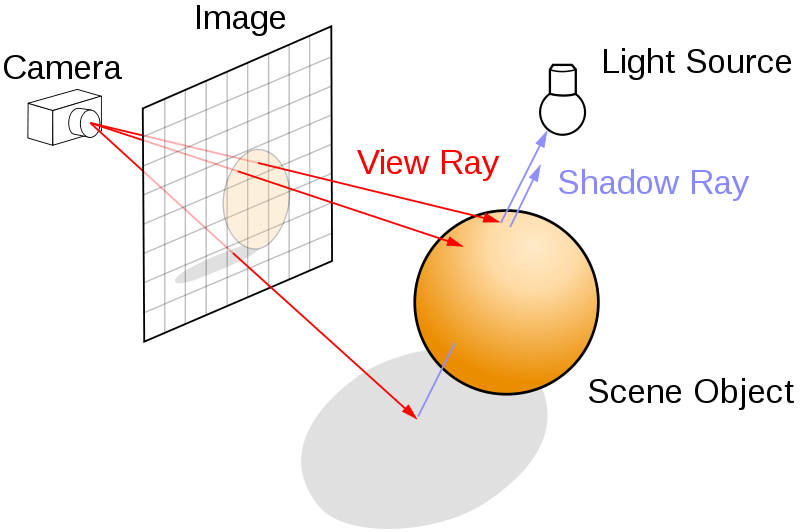
\includegraphics[height=3.0in]{figures/Ray_trace_diagram.png}
\caption{Ray Tracing Diagram\cite{RayTracingDiagram}}
\label{fig:raytracingdiagram}
\end{figure}

\section{Direct Illumination: Ray Casting}
\label{sec:RayCasting}
For this thesis, direct illumination encapsulates the ray casting process. Direct illumination will is referred to as illumination that emanates from a virtual light in a 3D scene that contributes to a 3D object's final color in addition to that object's material attributes.  Direct illumination also encompasses an image's shadowing information, which is an obstruction in the light ray-object intersection.

Ray casting, a term first introduced by Scott Roth in 1982, is the process of casting rays into a 3D scene, finding the closest intersection from the eye/camera through boolean operations, and returning the color value of that object\cite{Roth1982}.  By emulating the different properties of light based on the cosine of the normal vector and the normalized vector from the high point of the object to a light, semi-realistic results are produced.  Other, more cartoon-ish, effects are created using similar methods, most notably Gooch and Gooch shading.

For this research, the basic Phong model of shading was used to generate specular highlights on 3D objects. This model, which has been altered slightly by Jim Blinn, will be discussed fully in following sections.  The Phong model equation is for a ray intersecting the surface of an object at point ~$P$ as follows:

\begin{equation}
\label{eq:phongModel}
color_{output} = k_{d}O_{d}I_{a} + k_{d}O_{d}I_{d}[\hat{L_{m}} \cdot \hat{N}] + k_{s}O_{s}[\hat{R_{m}} \cdot \hat{V}]^{n}I_{d} \cite{hughes2013computer}
\end{equation}

where ~$k_{d}$ and ~$k_{s}$ are the diffuse and specular reflection coefficients, ~$I_{a}$ is the ambient light color, ~$I_{d}$ is the diffuse light color, ~$O_{d}$ is the diffuse color of the object, ~$L_m$ is the direction vector from point ~$P$ towards the light, ~$N$ is the surface normal for the surface at ~$P$, ~$O_{s}$ is the specular color of the object, ~$R_m$ is the direction that a perfectly reflected ray of light would take from ~$P$, and ~$n$ is the specular exponent, or shininess.  Each part of this equation will be discussed.  The second part of the equation,  ~$k_{d}O_{d}I_{d}[\hat{L_{m}} \cdot \hat{N}]$,  can be easily defined with Lambert shading.

\subsection{Lambert Shading}
\label{subsec: Lambert Shading}
\begin{figure}[h]
\centering
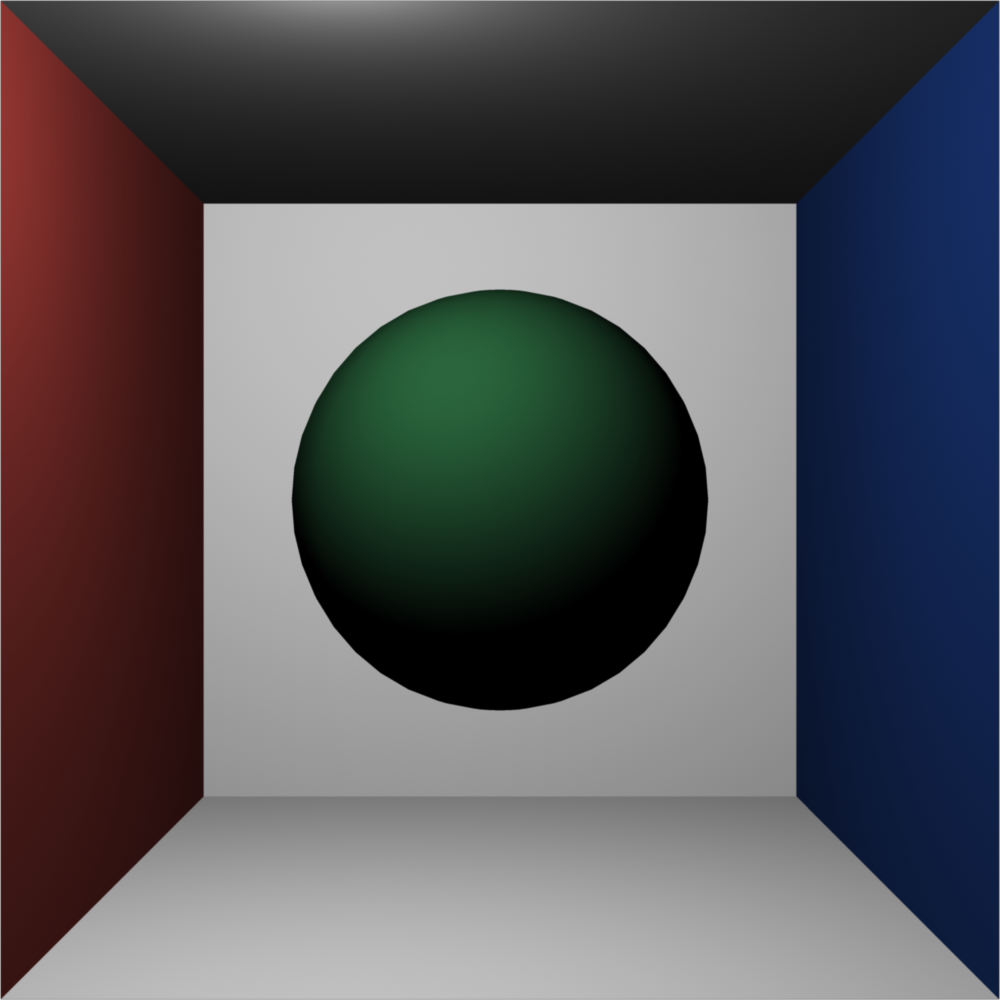
\includegraphics[height=3.0in]{figures/lambert_Maya.png}
\caption{An example of Lambert Shading created in Autodesk Maya 2010\copyright}
\label{fig:lambertmaya}
\end{figure}
The Lambertian model for reflectance is the diffuse component of a surface's material, or the diffuse reflection of a material's properties.  Diffuse objects are generally thought of as anything that does not reflect light off of its surface, such as unfinished wood.  This effect can be see in Figure \ref{fig:lambertmaya}. This model follows Lambert's cosine law for optics, which states that the radian intensity or luminous intensity observed from an ideal diffusely reflecting surface or ideal diffuse radiator is directly proportional to the cosine of the angle ~$\theta$ between the observer's line of sight and the surface normal.  Applying this law to computer graphics we the following equation:

\begin{equation}
\label{eq:lambert}
color_{output} = \hat{L_{m}} \cdot \hat{N} CI_{L}
\end{equation}

where ~$\hat{L_{m}}$ is the normalized direction of the light-direction vector, ~$\hat{N}$ is the normalized normal vector, ~$C$ is the color, and ~$I_{L}$ is the intensity of the incoming light.  Since ~$L \cdot N =  |N||L|\cos{\theta}$, if we make the lengths of ~$|N||L| = 1$ by normalizing them, equation \ref{eq:lambert} satisfies the properties for Lambertian shading by making ~$L \cdot N = \cos(\theta)$.  As we can see, Equation \ref{eq:lambert} is actually the term represented as ~$k_{d}O_{d}I_{d}[\hat{L_{m}} \cdot \hat{N}]$ in Equation \ref{eq:phongModel}, where ~$C = O_{d}$ and ~$I_{L} = I_{d}$.

\subsection{Gouraud Shading}
\label{subsec: Gouraud Shading}
One of the first shading paradigms introduced to the computer graphics community was a vertex interpolation shading created by Henrik Gouraud at the University of Utah\cite{gouraud1971}.  Gouraud's algorithm successfully captured the Lambertian Shading effect described in Section \ref{subsec: Lambert Shading}.  Gouraud's approach saved intensity values at each vertex as a weighted average of the normals of the surrounding polygons in the object's mesh.  When a hit on an object was achieved, a weighted sum of the point's color was returned depending on the intensity values at each closest vertex.  This effect is demonstrated in Figure \ref{fig:gouraudMaya}.
\begin{figure}[h]
\centering
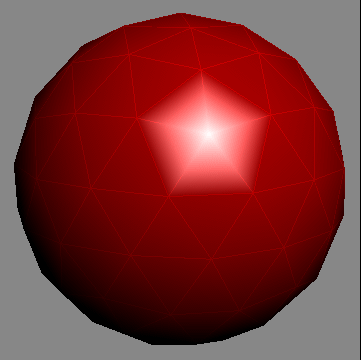
\includegraphics[height=3.0in]{figures/gouraud_low.png}
\caption{An example of the deficit of Gouraud shading being apparent in the highlight in a lowpoly model.\cite{GouraudLow} }
\label{fig:gouraudMaya}
\end{figure}

While this method works well,  it is also dependent on the density of the object's mesh since each vertex intensity is basically an average of the surrounding normals.  This technique also benefits from the relatively simple calculations needed per hit point because, generally speaking, a polygon is made up of a 3 or 4 vertexes maximum.  Instead of calculating Equation \ref{eq:phongModel} at each pixel of intersection within the scene, interpolation between precalculated vertex intensities is needed.  Unfortunately, since the smooth perception of shading is based off of interpolation, which in effect is characterized by the density of object meshes, high localized specular highlights will not be rendered correctly.  Also, if a highlight lies in the middle of a polygon, but does not spread to the polygon's vertex, it will not be apparent in the render.  If the highlight appears directly on a vertex, while it will be rendered correctly for that vertex, it will be rendered incorrectly on neighboring polygons. An example of this deficit for Gouraud's shading can be see in Figure \ref{fig:gouraudMaya}.  For this reason, Equation \ref{eq:phongModel} was introduced.

\subsection{Phong Shading}
\label{subsec:Phong Shading}
\begin{figure}[h]
\centering
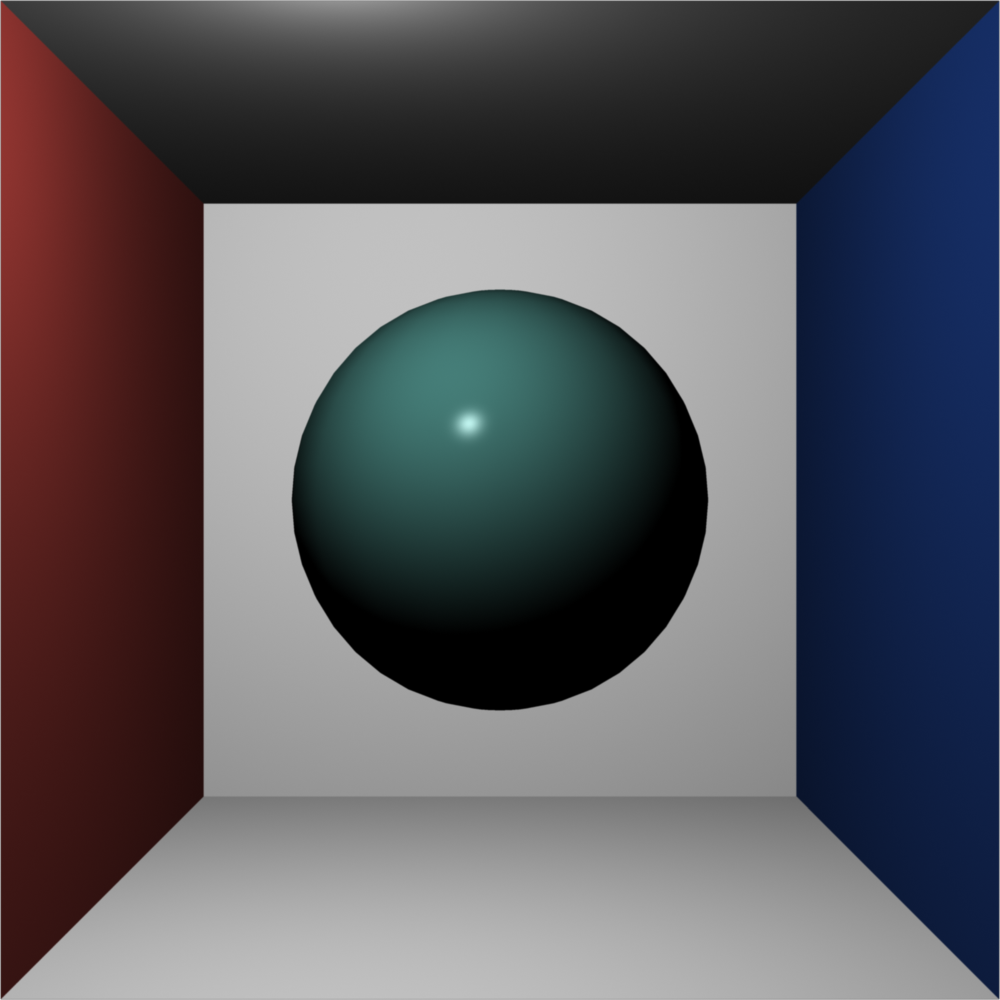
\includegraphics[height=3.0in]{figures/phong_Maya.png}
\caption{Phong Shading created in Autodesk Maya\copyright 2010}
\label{fig:phongmaya}
\end{figure}
Another aspect of an object's illumination model is the specular component of an object.  Specularity is the visual appearance of specular reflections.  This represents an object's ``shininess".  One strategy to display this specular highlight was introduced by Bui Tuong Phong \cite{Phong1975}. Whereas Phong's predecessors interpolated across surface patches \cite{gouraud1971}, as stated in Section \ref{subsec: Gouraud Shading}, Phong interpolated surface normals and evaluated a lighting model at each pixel.  He also added a specular component to the lighting model to produce highlights.\cite{lyon1993phong}

Phong's specular component from his paper \textit{Illumination for Computer-Generated Images} introduces the equation at ray-object intersection point ~$P$:

\begin{equation}
\label{eq:Phong01}
color = C_{p}[\cos{i} + d] + W(i)[\cos{s}]^{n}
\end{equation}

where~$C_p$ is the reflection coefficient of the object at point ~$P$,~$i$ is the incident angle,~$d$ is the environmental diffuse reflection coefficient, ~$W(i)$ is a function which gives the ratio of the specular reflected light and the incident light as a function of the incident angle ~$i$, and ~$s$ is the angle between the direction of the reflected light and the light of sight.

The important aspect of Equation \ref{eq:Phong01} is the term ~$[\cos(s)]^{n}$.  Since the cosine of the angle between the direction of the reflected light, or ~$R_{m}$ in Equation \ref{eq:phongModel}, and the line of sight, ~$V$, is equal to ~$R_{m} \cdot V$ as long as each vector is of unit length, we only need to know what ~$R_{m}$ is.

To calculate ~$R_{m}$ we have this equation from Phong as well\cite{lyon1993phong} at ray-object intersection point ~$P$:
\begin{equation}
\label{eq:phongreflect}
R_m = 2[L_m \cdot N]N - L_m
\end{equation}

where ~$L_{m}$ is the direction vector from ~$P$ towards the light and ~$N$ is the surface normal at ~$P$.  The effect of Phong shading can be seen in Figure \ref{fig:phongmaya}.

\subsection{Blinn Shading}
\label{subsec:Blinn Shading}
\begin{figure}[h]
\centering
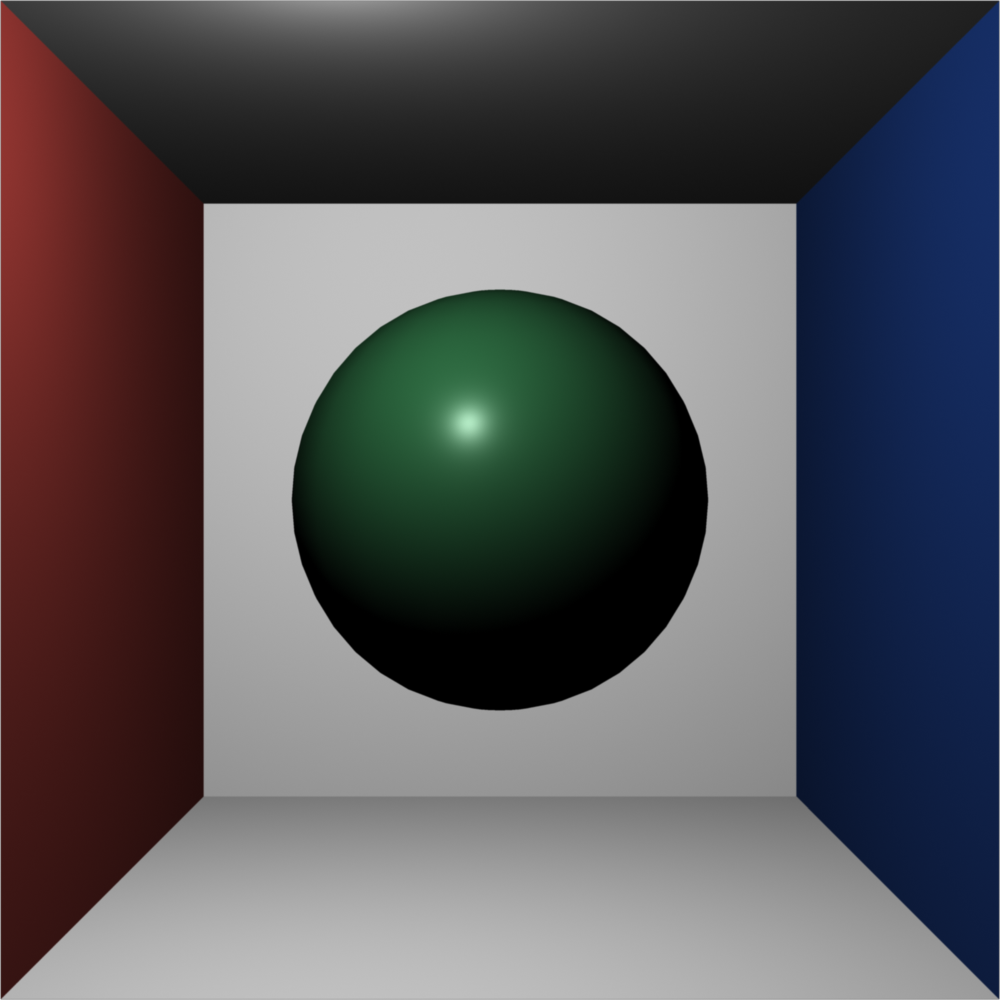
\includegraphics[height=3.0in]{figures/blinn_Maya.png}
\caption{Blinn Shading created in Autodesk Maya 2010\copyright}
\label{fig:gooch}
\end{figure}
In Jim Blinn's paper \textit{Models of Light Reflection for Computer Synthesized Pictures} he introduces the equation\cite{Blinn:1977}:

\begin{equation}
\label{eq:blinnModel01}
color = p_{a} + max(0,N\cdot L) p_{d} +  (N \cdot H)^n p_{s}
\end{equation}
which is most similar to Equation \ref{eq:phongModel} because of its ambient term ~$p_{a}$, diffuse term ~$p_{d}$ and specular term ~$p_{s}$.  Most importantly for Blinn's equation is the inclusion of ~$H$.  Instead of using Phong's ~$R_{m}$ from Equation \ref{eq:phongreflect}, Blinn introduces a new half-vector called ~$H$.  Blinn describes,

\begin{quote}
``If the surface was a perfect mirror, light would only reach the eye if the surface normal, ~$N$, pointed halfway between the source direction, ~$L$, and the eye direction, ~$E$.  We will name this direction of maximum hilights ~$H$..."
\end{quote}
Relating this to the variables in this paper:
\begin{equation}
\label{eq:BlinnH}
H = \frac{\hat{L} + \hat{V}}{len(L+V)}
\end{equation}

Equation \ref{eq:BlinnH} then replaces ~$R \cdot V$ in Equation \ref{eq:phongModel}.  Blinn's model produces more accurate models of empirically determined  bidirectional reflectance distribution functions for many different types of surfaces\cite{ngan2004experimental}.  While this equation produces better results, it also introduces a square root math function when determining  ~$len(L+V)$.  Since a square root calculation takes more time than a dot product calculation, Blinn's model has been considered slower.(With computer processing achievements today, however, the speed differences are incomparable.)  Although it will not be used in this thesis, I hvae included it to help show the origins of Equation \ref{eq:phongModel}.

\subsection{Gooch and Gooch Shading}
\label{subsec:GoochShading}
\begin{figure}[h]
\centering
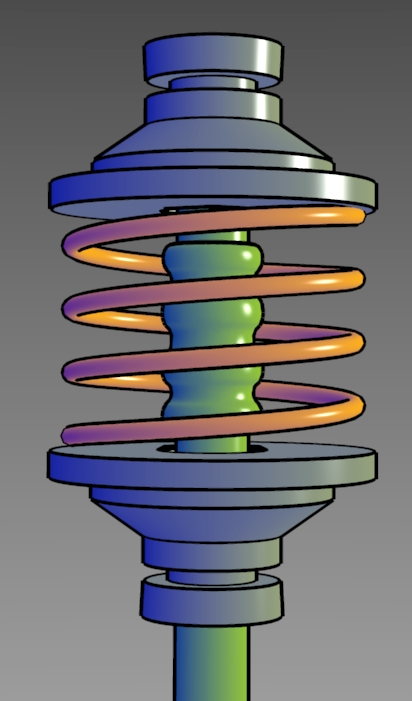
\includegraphics[height=3.0in]{figures/gooch.jpg}
\caption{Gooch Shading Example\cite{gooch1998non}}
\label{fig:gooch}
\end{figure}
Ever since the introduction of Phong's model for photo-realistic rendering of geometric objects, there has been a trend towards non-photorealistic rendering(NPR).  Most notable in this field is the work of Amy and Bruce Gooch, et al.  Gooch and Gooch argue that ``Phong shaded 3D imagery does not provide geometric information of the same richness as human-drawn technical illustration\cite{gooch1998non}."    NPR techniques are referred to as computer graphics algorithms that imitate traditional techniques such as painting or pen-and-ink\cite{gooch1998non}.  Gooch, et al. introduced a generalization of the classic computer graphics equation from Equation \ref{eq:lambert} by experimenting with the value of ~$L_{m} \cdot N$.  Their equation is as follows:

\begin{equation}
\label{eq:Gooch&Gooch}
color = \left(\frac{1 + (\hat{L_{m}} \cdot \hat{N})}{2}\right) k_{cool} + \left(1-\frac{1 + (\hat{L_{m}} \cdot \hat{N})}{2}\right) k_{warm}
\end{equation}
where ~$k_{cool}$ and ~$k_{warm}$ are two color values to interpolate between. In Equation \ref{eq:Gooch&Gooch}, they use the large fractions to remap the values of ~$\hat{L_{m}} \cdot \hat{N}$ between zero and one, causing the colors to gracefully blend from ~$k_{cool}$ to ~$k_{warm}$.  As can be seen in Figure \ref{fig:gooch}, the Gooch shading algorithm also includes outlines around each shape.  Gooch referred to creating the outline in the paper \textit{Real-Time Nonphotorealistic Rendering}\cite{markosian1997real}, but for this thesis the outline is determined from when the values of ~$\hat{L_{m}} \cdot \hat{N}$, after being remapped between 0 and 1, are between a certain threshold and zero.  While this may not the best way to generate outlines around 3D shapes, it accomplishes semi-reliable results and was therefore utilized in this thesis.
\subsection{Texture Mapping and UV Coordinates}
\label{subsec:TexMap}
\begin{figure}[h]
\centering
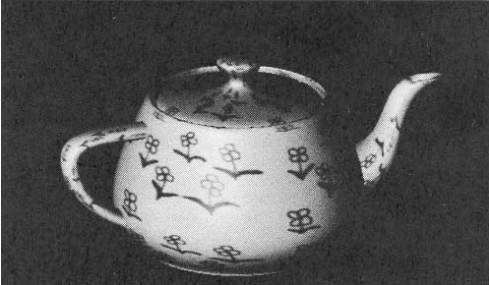
\includegraphics[height=2.0in]{figures/flowerteapot.png}
\caption{An example of texture mapping to the surface of a teapot. \cite{blinn1976texture}}
\label{fig:teapot}
\end{figure}
Up to this point, we've focused on explaining basic color appropriation with solid colors represented as RGB; in computer graphics,however, it is also possible to map photographs to the surface of 3D objects.  This idea was first introduced by Ed Catmull in 1974 when he demonstrated a method of representing 3D curved patches as opposed to conventional polygons.  This method ``maps" photographs to the surfaces of these patches\cite{catmull1974subdivision}. Jim Blinn expanded this to include environmental mapping based off of reflections from the surface of objects\cite{blinn1976texture}, as can be seen in Figure \ref{fig:teapot}.

\subsubsection{Bump/Normal Mapping}
\label{subsubsec:BNMap}
\begin{figure}[h]
\centering
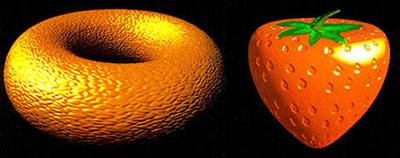
\includegraphics[height=2.0in]{figures/blinn_bump.jpg}
\caption{An example of bump mapping introduced by Jim Blinn. \cite{blinn1978simulation}}
\label{fig:bumpmap}
\end{figure}
As another expansion of Catmull's texture mapping, Blinn also introduced a technique that could simulate a rough or textured surface on a 3D shape, called bump mapping\cite{blinn1976texture}. Blinn discovered that by altering the normal at each point of intersection on the surface of a 3D shape, simulations of wrinkled surfaces can be generated as seen in Figure \ref{fig:bumpmap}.  The normal at each point can be mapped to an image texture or altered via a noise generating equation such as Perlin noise.  Blinn's wrinkled surface simulation can be seen in Figure \ref{fig:bumpmap}.
\section{Ray Tracing and Distributed Ray Tracing}
To improve upon the Phong specular shading model, a new recursive technique was introduced by Turner Whitted at Bell Laboratories.  Turner hypothesized that a tree model should be used to calculate accurate, realistic representations of the physical world's reflective process.  He based his algorithm on an reflection ray, ~$R$, that represents the reflection of a ray on a perfectly smooth surface, and ~$P$, which represents the transmitted ray through a perfectly smooth surface:

\begin{equation}
\label{eq:raytracing1}
\hat{V}' = \frac{\hat{V}}{\hat{V} \cdot \hat{N}}
\end{equation}
\begin{equation}
\label{eq:raytracing2}
\hat{R} = \hat{V}' + 2\hat{N}
\end{equation}
\begin{equation}
\label{eq:raytracing3}
\hat{P} = k_{f}(\hat{N} + \hat{V}') - \hat{N}
\end{equation}
where
\begin{equation}
\label{eq:raytracing4}
k_{f} = (k_{n}^{2}|\hat{V}'|^{2} - |\hat{V}' + \hat{N}'|^2)^{\frac{1}{2}}
\end{equation}

and $k_{n}$ is the index of refraction for the surface.  The equations assume that ${\hat{V} \cdot \hat{N}}$ is less than zero so the sign of ${N}$ must also be adjusted to point to the side of the surface the intersecting angle is incident from. When tracing a ray from the eye point, the intersection at each reflective surface determines the next surface hit, forming a recursive tree formation.  Upon achieving this tree, the following equation calculates the surface color:

\begin{equation}
\label{eq:raytracing5}
color_{output} = I_{a} + k_{d} \sum{j=1}^{j=ls}(\hat{N} \cdot \hat{L_{j}}) + k_{s}S + k_{t}T
\end{equation}
where \newline
\noindent
$S$ = the intensity of light incident from the $\hat{R}$ direction\newline
$k_{t}$ = the transmission coefficient\newline
$T$ = the intensity of light from the $\hat{P}$ direction\newline

By keeping $k_{s}$ and $k_{t}$ constant Turner achieved his results, but for ideal cirumstances the values should be mapped to a Fresnel algorithm that relates them to realistic models of reflection and refraction.

To enhance the raytracing process, Cook, Loren and Carpenter introduced the term ``distributed ray tracing", described as:

\begin{quote}
``...The key is that no extra rays are needed beyond those used for oversampling in space.  For example, rather than taking multiple time samples at every spacial location, the rays are distributed in time so that rays at different spatial locations are traced at different instants of time.
\begin{itemize}
\item Sampling the reflected ray according to the specular distribution function produces gloss (blurred reflection)
\item Sampling the transmitted ray produces translucency (blurred transparency).
\item Sampling the solid angle of the light sources produces penumbras.
\item Sampling the camera lens area produces depth of field.
\item Sampling in time produces motion blur."
\end{itemize}
\end{quote}

The introduction of randomization, or jittering, achieves the distributed ray tracing effect. By jittering the ${R}$ value of $T$ in Equation \ref{eq:raytracing5} a glossy effect is produced. The same can be said of the $P$ value from the $T$ variable in Equation \ref{eq:raytracing5}.  Distributed ray tracing is important to a 3D image's realism because it is not possible to achieve the computed perfect reflection/refraction model introduced by Whitted in the natural world.

\section{Indirect Illumination/ Radiosity Effects}
For this thesis, Indirect illumination accounts for any shading or color values not calculated directly from the virtual light in a scene.   These terms are known as ambient occlusion, global illumination and caustic effects. In the natural world, diffuse reflection is the reflection of light from a surface such that an incident ray is reflected at many angles rather than at just one angle, which is the case of specular reflection.  Typically an object will base its final color off of not only the light shining at it, but also from the colors of the objects in closest proximity to it.  This effect is seen in Figure \ref{fig:diffusereflectionrw} in the picture of a racquetball.  The surface of both the racquetball and the piece of paper are as close to Lambertian surfaces as can be found in the natural world.  In the figure the diffuse reflection is most prominent in the racquetball's shadow.  It may seem like a trick on the eyes, but the shadow has a purple tint to it because of the diffusely reflected light rays coming from the racquetball.  In theory, if an object is illuminated in a room with bright red walls the color of the object will have a red tint because of the diffuse reflection of the red from the walls contributing to the overall color of its surface.  It is near impossible to determine all the different contributors to an objects final color in the natural world because of the infinite amount of light rays absorbed and reflected by an object's surface.

\begin{figure}[h]
\centering
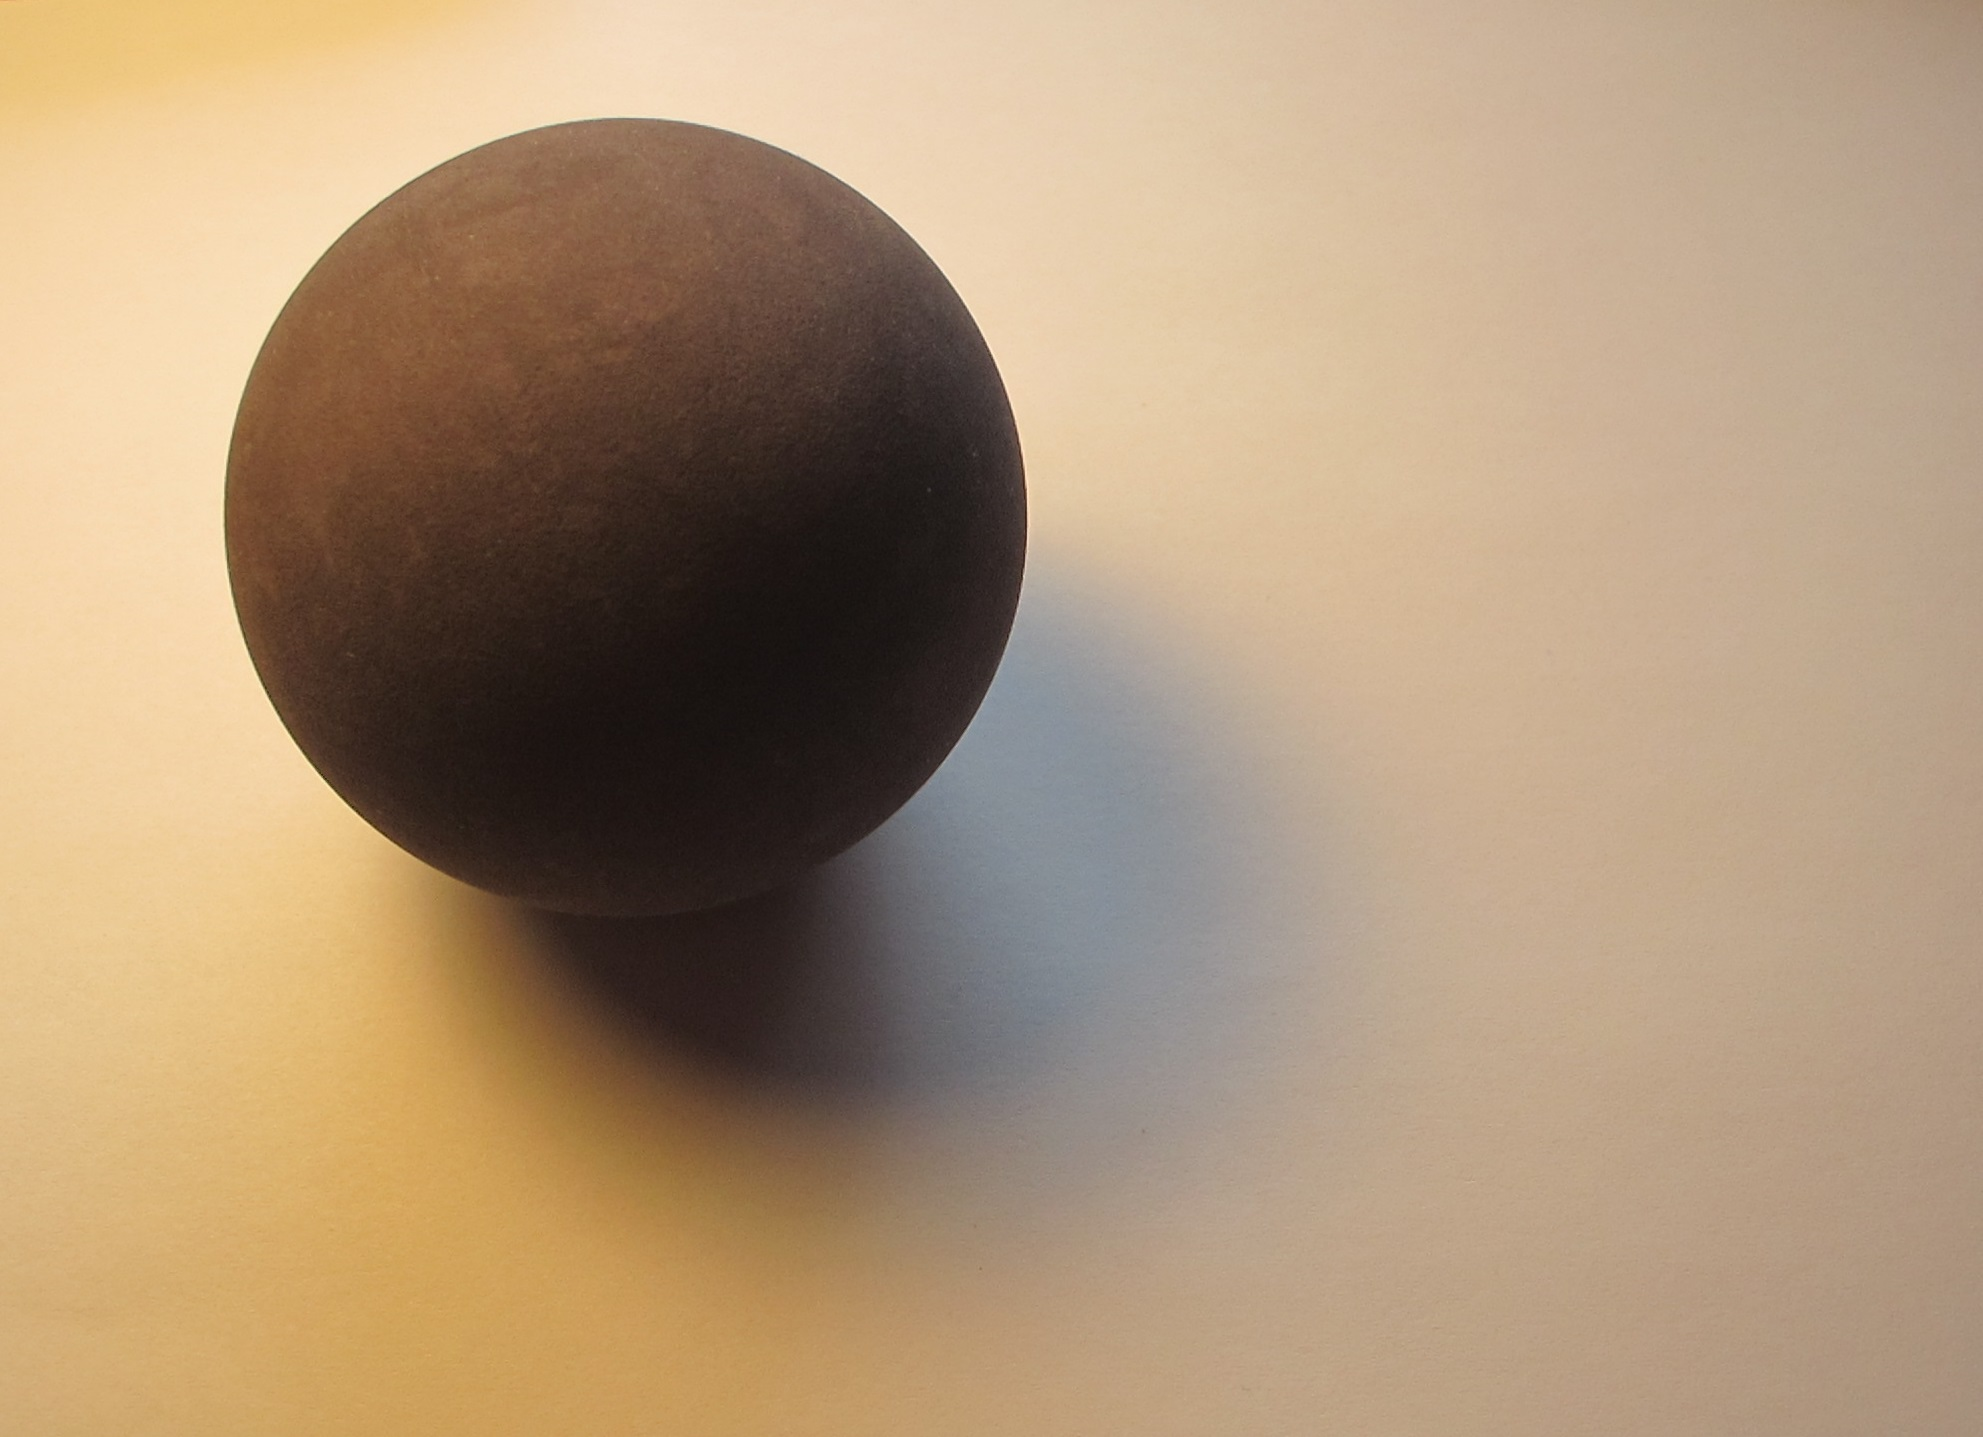
\includegraphics[height=3.0in]{figures/raquetball.JPG}
\caption{Real World Indirect Illumination/Radiosity Effect with a racquetball on a piece of paper.}
\label{fig:diffusereflectionrw}
\end{figure}

To simulate this effect in a 3D environment, new terms were introduced by Torrance, Greenberg et.al \cite{Goral:1984}, who determined a model of light interaction between diffuse surfaces based off of methods used in thermal engineering.  To simplify their method, this thesis used a method inspired by their work.  The process to calculate ambient occulsion, global illumination, and caustic effects are fundamentally all the same.  At each point in a scene, a specific number of sample rays will be cast at each intersection point.  The average of the resulting color information from each sampling ray set determines that pixel's final color.  Ambient occlusion is the simplest.  Ambient occlusion informs the proximity of objects with other objects.  Ambient Occlusions produces a black and white image that will be darker in pixels where images are closer together and lighter in places where images are farther apart.  To calculate this set, one simply needs to determine if another object is hit by a ray in the set or not.  For instance, if 255 rays are cast from an object, and 200 of them hit another object in a distance greater than 0, then the value for that pixel will be 200/255 or .7843.  An ambient occlusion example can be seen in Figure \ref{fig:aOcclusion}.

\begin{figure}[h]
\centering
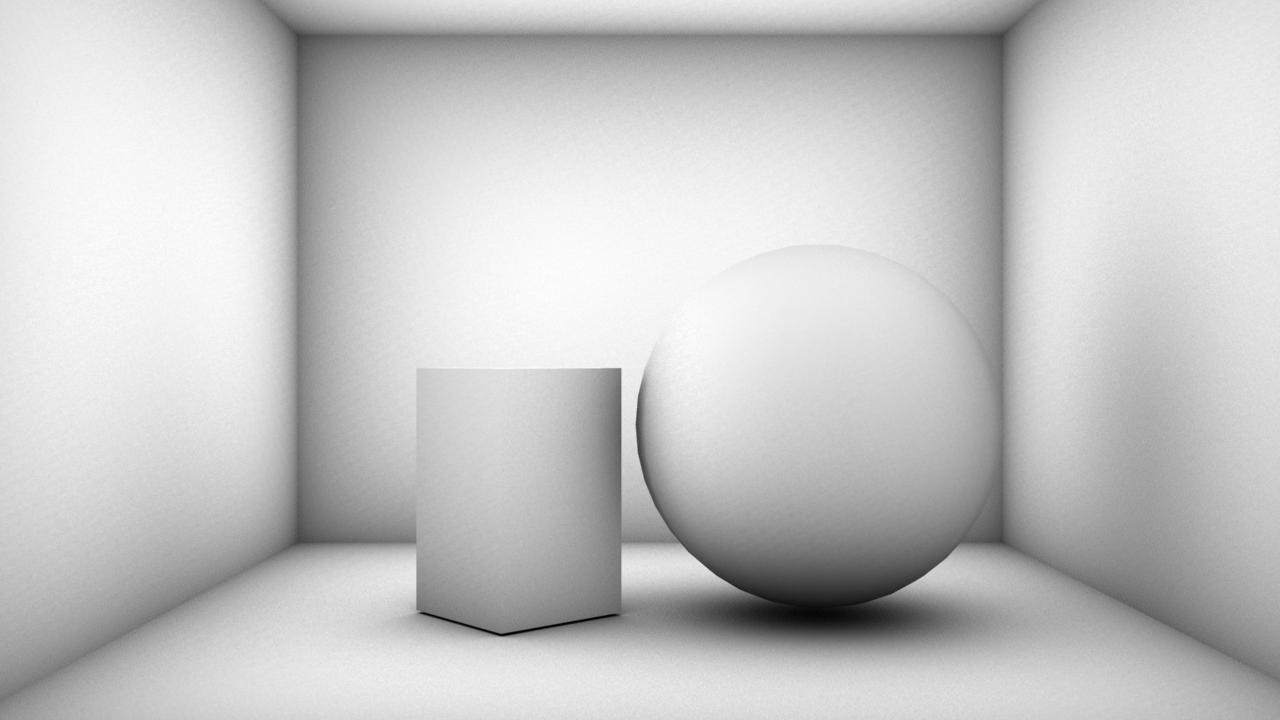
\includegraphics[height=3.0in]{figures/aOcclusion.jpg}
\caption{Example of Ambient Occlusion}
\label{fig:aOcclusion}
\end{figure}

To calculate global illumination, at each point in the sample set of data, instead of calculating the distance from the point, the direct illumination shading value is added.  Rather than the average number of intersections, the average color is determined from 255 sample rays for a global illumination calculation.  This is seen in Figure \ref{fig:globalill}.  This process is where the color bleeding from nearby objects can best be seen.

\begin{figure}[h]
\centering
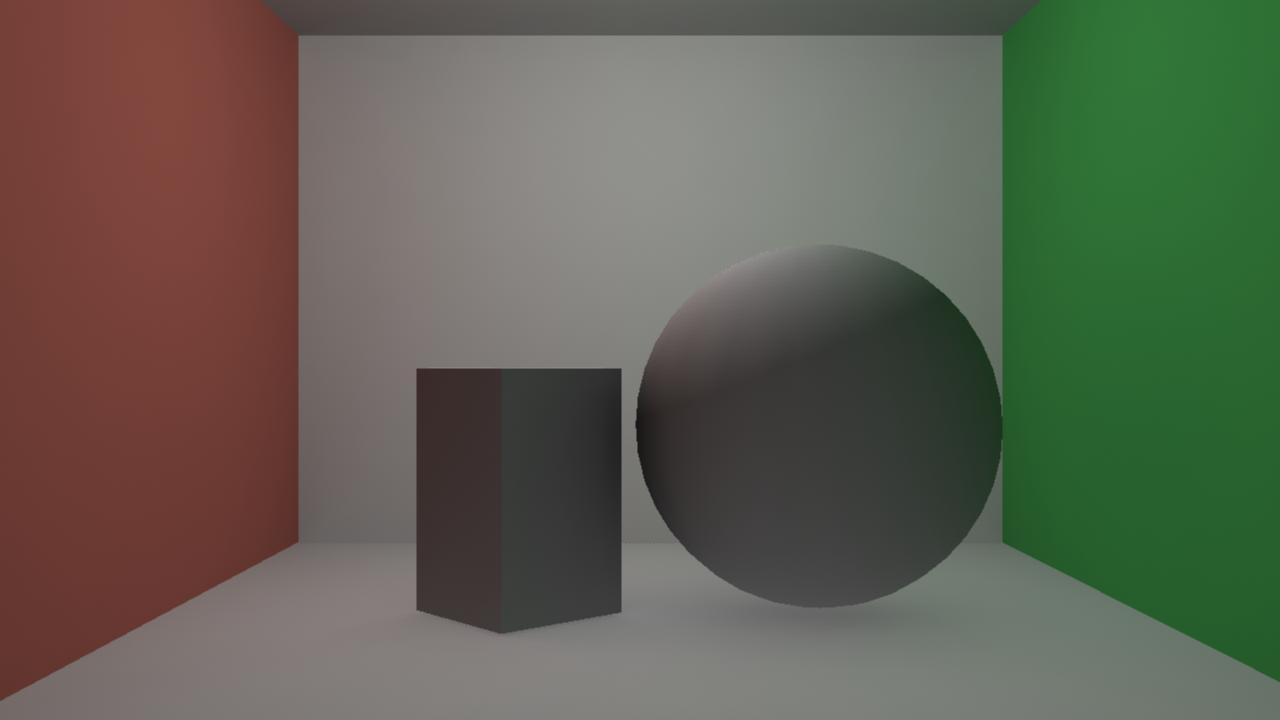
\includegraphics[height=3.0in]{figures/globalIll.jpg}
\caption{Example of Global Illumination}
\label{fig:globalill}
\end{figure}

The final effect is a caustic, which is the ratio of specular color at each point on a surface.  If a surface receives caustics, it calculates the reflective rays of nearby objects and returns the reflected color value average for each sample ray set.  This effect is seen in Figure \ref{fig:caustics}.
\begin{figure}[h]
\centering
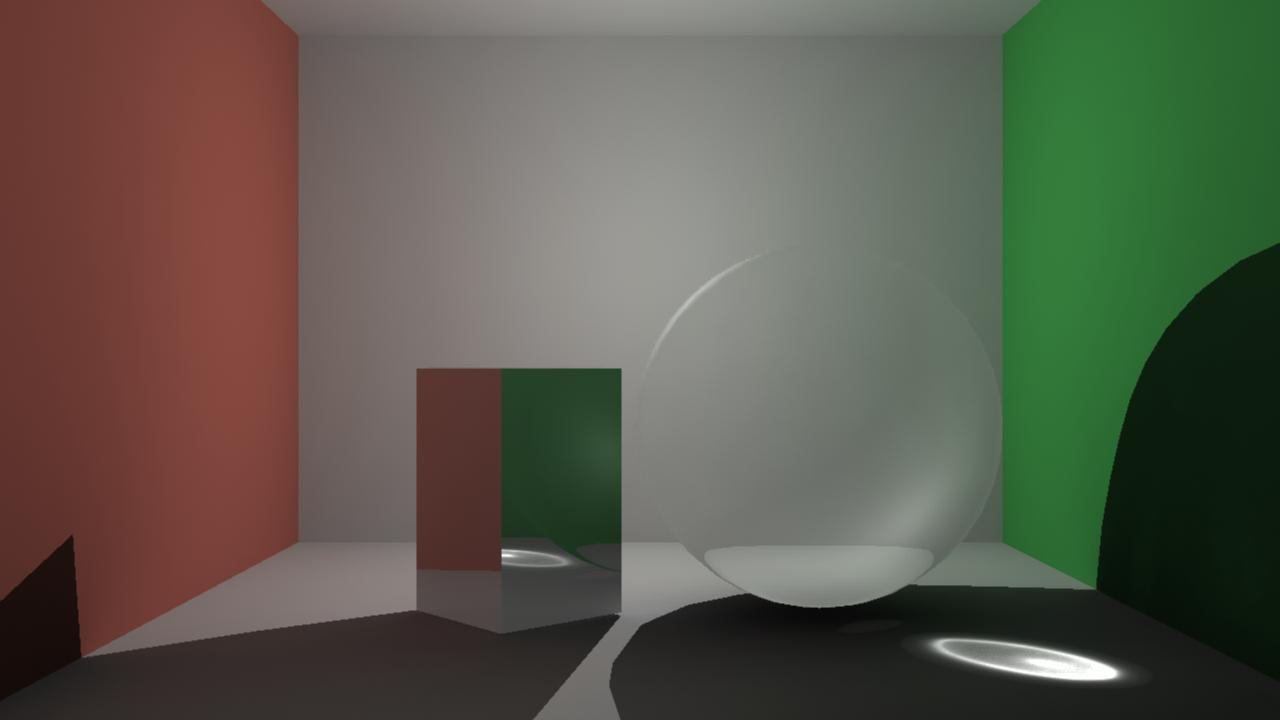
\includegraphics[height=3.0in]{figures/caustics.jpg}
\caption{Example of Caustic Effect}
\label{fig:caustics}
\end{figure}

Indirect illumination combined with distributed ray tracing has made a difference in the realistic perception of generated photorealistic images, and an effort is being made to incorporate these effects into realtime settings like video games in order to provide a more immersive experience.  Large sample ray sets are needed for more realistic looking images however, and the computing power required to produce this effect in realtime is sizable and expensive.

\section{Languages}
The four languages I evaluated were determined for specific reasons.  They had to have the ability to follow the object-oriented paradigm and possess the potential to perform graphical methods like imaged reading and writing.  A brief history behind each language will be discussed to give insight into the basis for each language's creation, which will also provide insight as to their feasibility in creating an image synthesis program.
\subsection{C++}
\label{sub:C++}
C++ is a general-purpose object-oriented coding language.  Its genesis lies in research done with the programming \textit{C with Classes} in 1979, although its commercial release was not until October 1985\cite{stroustrup1996history}. C++ is considered an intermediate-level language because of its capabilities with both high and low level computer functionality.  Creator Bjarne Stroustrup claims to have drawn inspiration from not only C, but also from Simula, Algol68, BCPL, Ada, CLU and ML.  Since its creation, C++ has gone on to influence the creation of numerous coding languages, such as C\#\cite{naugler2007c}.

According to Stroustrup, C++ was originally designed to combine Simula's facilities for program organization with C's efficiency and flexibility for systems programming\cite{stroustrup1996history}.  C++ is an extension of the C programming language. In fact, it stemmed from a fundamental design called \textit{C with Classes}\cite{stroustrup1996history}.  When Stroustrup designed the C++ language he had a variety of guidelines he deemed as ``suitable" for computer languages.  He writes:
\begin{quote}
\label{qt: StroustrupC++History}
\begin{enumerate}[label = {[\arabic*]}]
\item `` A good tool would have Simula's support for program organization- that is, classes, some form of class hierarchies, some form of support for concurrency, and strong(that is, static) checking of a type system based on classes.  This I saw as support for the process of inventing programs, as support for design rather than just support for implementation.

 \item A good tool would produce programs that ran as fast as BCPL programs and share BCPL's ability to easily combine separately compiled units into a program.  A simple linkage convention is essential for combining units written in languages such as C, Algol168, Fortran, BCPL, assembler, etc., into a single program and thus not get caught by inherent limitation in a single language

 \item A good tool should also allow for highly portable implementations.  My experience was the ``good" implementation I needed would typically not be available until ``next" year and only on a machine I couldn't afford....\cite{stroustrup1996history}"
\end{enumerate}
\end{quote}
To further emphasize C++'s benefits, Stroustrup explained why he chose C over other languages of the time to build upon:
\begin{quote}
\label{q:StroustrupCvsOther}
``C is clearly not the cleanest language ever designed nor the easiest to use so why do so many people use it?
\begin{enumerate}[label = {[\arabic*]}]
\item C is \textit{flexible}: It is possible to apply C to most every application area, and to use most every programming technique with C.  The language has no inherent limitations that preclude particular kinds of programs from being written.
\item C is \textit{efficient}:The semantics of C are ``low level"; that is, the fundamental concepts of C mirror the fundamental concepts of a traditional computer.  Consequently, it is relatively easy for a compiler and/or a programmer to efficiently utilize hardware resources for a C program.
\item C is \textit{available}: Given a computer, whether the tiniest micro or the largest super-computer, the chance is that there is an acceptable quality C compiler available and that that C compiler supports an acceptably complete and standard C language and library.  There are also library and support tools available, so that a programmer rarely needs to design a new system from scratch.
\item C is \textit{portable}: A C program is not automatically portable from one machine (and operating system) to another nor is such a port necessarily easy to do.  It is, however, usually possible and the level of difficulty is such that porting even major pieces of software with inherent machine dependencies is typically technically and economically feasible.
\end{enumerate}
Compared with these ``first order" advantages, the ``second order" drawbacks like the curious C declarator syntax and the lack of safety of some language constructs become less important. Designing ``a better C" implies compensating for the major problems involved in writing, debugging, and maintaining C programs without compromising the advantages of C. C++ preserves all these advantages and compatibility with C at the cost of abandoning claims to perfection and of some compiler and language complexity. However, designing a language ``from scratch" does not ensure perfection, and the C++ compilers compare favorably in run−time, have better error detection and reporting, and equal the C compilers in code quality. \cite{stroustrup1996history}"
\end{quote}
Stroustrup sought to create a universal, object-oriented language that was accessible and relatively low maintenance to begin programming with since most computers were, and still are, compatible with C.

Object-oriented programming provides clean and modular code that is easier to maintain and debug, because it separates functions and utilities into class objects, which can be reused.  This is C++'s main benefit to the image synthesis process, in addition to its efficiency in utilizing hardware resources from a computer to provide faster results.

\subsection{Processing}
\label{sub:Processing}
Processing is an open-source programming language and integrated development environment, or IDE, developed by Casey Reas and Benjamin Fry in 2001. According to the Processing website (processing.org):
\begin{quote}
``Processing is a programming language, development environment, and online community.  Since 2001, Processing has promoted software literacy within the visual arts and visual literacy within technology.  Initially created to serve as a software sketchbook and to teach computer programming within a visual context, Processing evolved into a development tool for professionals.  Today there are tens of thousands of students, artists, designers, researchers and hobbyists who use Processing for learning, prototyping and production."
\end{quote}

Andrew Glassner, a pioneer in Ray Tracing, also wrote a book on Processing called \textit{Processing for Visual Artists}.  Glassner helps to emphasize the importance and use for Processing in the visual world:

\begin{quote}
``Processing is for artists, designers, visualization creators, hobbyists or anyone else looking to create images, animation, and interactive pieces for art, education, science or business....Processing offers you a 21st-century medium for expressing new kinds of ideas and engaging audiences in new ways..."
\end{quote}

The usefulness and applicability of Processing in the ray tracing process can be found in its mission statement. It was initially designed to teach computer programming within a visual context.  Since that is also the aim and goal of this thesis, Processing was a reasonable option to investigate. Processing uses Java syntax and packages the java compilation process into its IDE, so a functional overview of Java is also needed to fully determine the usefullness of Processing.

\subsubsection{Java}
%TODO Object-oriented - high Level - cross platform

\subsection{Python}
\label{sub:Python}
Python, named after \textit{Monty Python's Flying Circus}, was first founded by Guido van Rossum.  He began his work on Python at the the National Research Institute for Mathematics and Computer Science in the Netherlands in 1989.  Python is a high-level and interpreted programming language.  While it can be argued that all computer languages are interpreted, Python is considered an interpreted language because unlike C or C++, Python does not require a compiler to operate.  While C and C++ compiled code needs to be compiled into machine-language before it is relayed to the computer, Python's instructions are interpreted directly from its written code.  van Rossum is quoted as saying he was unhappy with the productivity of creating a script or utility in C, which influenced his interest in establishing Python\cite{vanBlog1}.

One of the main focuses of Python is readable syntax.  According to Jim Mcconnell's book \textit{Code Complete}, one line of Python is equivalent to six lines of C code\cite{mcconnell2004code}.  According to van Rossum, Python's creation was heavily influenced by the coding language ABC.  ABC's design was intended to be a programming language that could be taught to intelligent computer users who were not computer programmers or software developers.  The main deficit with ABC's design was its inability to bridge the gap in GUI creation and an inability to directly access the file system and operating system in a computer.  Python's syntax eliminates the need for traditional curly braces (\{\}) and instead uses a tabular system that denotes code blocks.
\subsection{RenderMan}
\label{sub:RenderMan}
RenderMan\copyright\space is a software and application programming interface, or API, that many companies in the computer industry use to render large projects for entertainment or video game use.  RenderMan\copyright\space specializes in network distribution of renderings throughout a ``renderfarm" that has the ability to render ray traced images faster than a single computer.  RenderMan\copyright\space is referred to as the rendering engine that produces the image.  RenderMan\copyright\space is dependent on two files: RenderMan\copyright\space Interface Bytestream (RIB) and RenderMan\copyright\space shading file.  RIB acts as a descriptor for how the engine should work, incorporating all aspects of ray casting, ray tracing, direct illumination, distributed ray casting, and direct illumination.  A shading file is written in the RenderMan\copyright\space Shading Language (RSL), and acts as a description file for how objects in a scene interact with light.  By utilizing the RIB and RSL files, each ray tracing milestone was accomplished within the scope of this thesis.

It is important to note that RenderMan\copyright\space has already implemented all of the milestones needed for this thesis.  Also, RenderMan\copyright\space is based off of a camera projection matrix algorithm that does not cast rays the same way that this thesis does ray casting.  RenderMan\copyright\space also incorporates a variety of highly advanced rendering techniques that are too far outside the scope of this modest master's thesis to discuss.  The thesis will discuss the feasibility of utilizing the pre-constructed implementations of the milestones without the aid of production software such as Autodesk Maya\copyright\space or  Side Effects Houdini\copyright\space. This will present the same types of implementation issues that C++, Processing, and Python would in regards to the theory of ray casting. 